\input{../../common/latex_asst_template/asst_template.tex}

\class{ECEN 625}
\term{Winter 2021}
\assttitle{Lab 0: Setup}
\duedate{TBD}


\setuppage

\begin{document}

\maketitle
\thispagestyle{fancy}

\section{Tutorials} 
In this class you are expected to be familiar with the Linux command line, Git and Github.  If you haven't used these tools before, here are links to a few tutorials:
\begin{itemize}
	\item \url{https://ryanstutorials.net/linuxtutorial/}
	\item \href{https://www.youtube.com/watch?v=USjZcfj8yxE}{Learn Git in 15 minutes}
	\item \href{https://www.youtube.com/watch?v=nhNq2kIvi9s}{Learn Github in 20 minutes}
\end{itemize}

\section{Set up your environment}
The assignments assume you are running an Ubuntu 18.04 Linux Operating System.  You may be able to complete some assignments on other Linux variants; however, for the assignments that use the Xilinx Vivado tools, you will likely need Ubuntu 18 LTS, but Ubuntu 16 or 20 LTS may work as well.

If you don't yet have a Linux OS environment set up, I would suggest doing so for use in this assignment, and subsequent assignments. VMWare Workstation is available for free to BYU students through CAEDM. You can also install a full Ubuntu image (including Xilinx tools) in Windows using WSL2.  \textbf{Alternatively, I have a machine available that you can ssh into -- if you want to go this route, please email me your desired username and I will create a login for you.}

\section{Tools}
You are welcome to use whatever development tools you like, but a few things I suggest you look into:
\begin{itemize}
    \item VS Code for code editing.
    \item Using SSH keys with Github to avoid having to enter your password when pushing your code up.
\end{itemize}

\section{Get the Class Code Repository}
\begin{enumerate}
	\item You must use this invitation link to set up a Github classroom repo for the class: \url{https://classroom.github.com/a/B3CVEv7k}
	\item This will create a blank repository for you.  On the github website for your repo, click the \textbf{Import Code} button (shown below), and import from \texttt{https://github.com/byu-cpe/ecen625\_student}.
	\begin{figure}[h!]
		\centering
		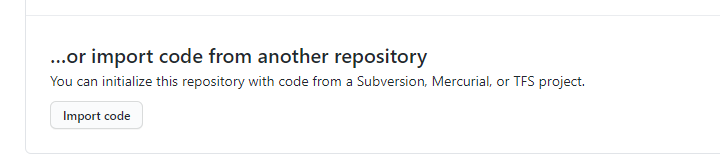
\includegraphics[width=0.8\textwidth]{import_code.png}
	\end{figure}
	\item Clone your repository to your local machine.  
\end{enumerate}

\end{document}